\documentclass[12pt]{article}

\usepackage[dvips,letterpaper,margin=0.75in,bottom=0.5in]{geometry}
\usepackage{cite}
\usepackage{slashed}
\usepackage{graphicx}
\usepackage{amsmath}
\usepackage{braket}
\begin{document}

\title{Analysis of Experimental Data}
\author{Michael Mulhearn}

\maketitle

\section{Statistical Distributions}

\subsection{Statistics of Experiments}

A primary purpose of science is to predict the results of experiments.  Consider a simple experiment with five possible outcomes which we repeat ten times.  If our theoretical prediction is that each of these five outcomes is equally probable, than our prediction for a typical series of ten experiments would be for each outcome to occur two times.  Now suppose we perform the experiment ten times and present the results like this:

\begin{figure}[htbp]
\begin{center}
{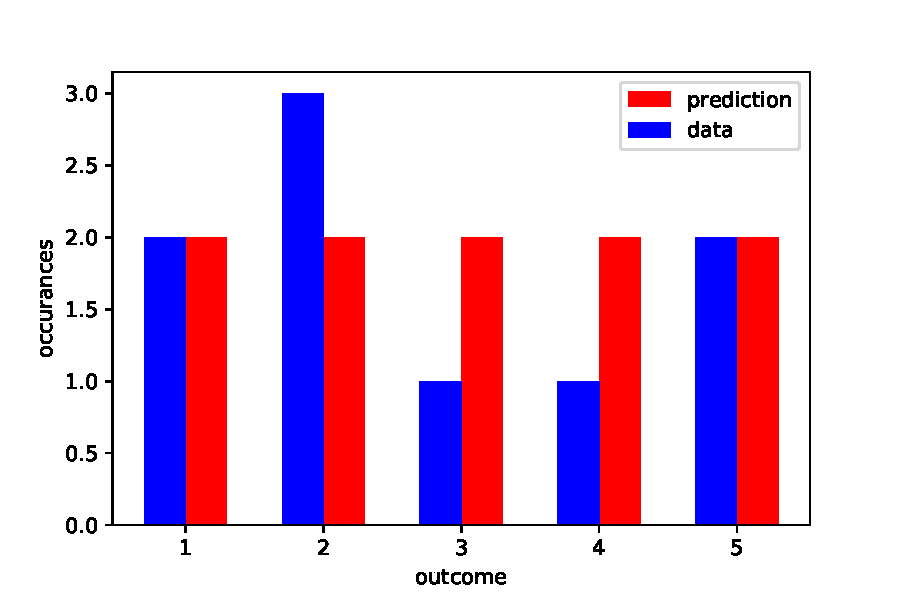
\includegraphics[width=0.45\textwidth]{figs/intro.pdf}}
\end{center}
\caption{\label{fig:intro} Comparison of experimental results with a prediction.}
\end{figure}

Scientist almost never display experimental data this way (as a bar graph) because it is nearly impossible to answer the crucial question {\em is this data consistent with this prediction?}  Even if every outcome has an equal probability, the results of individual experiments experience statistical fluctuations.  So even if the theory is correct, we well seldom reproduce exactly the theory prediction.

To interpret scientific experiments, it isn't enough to have a single prediction for the outcome of an experiment, instead, you need a prediction for the statistical distribution of outcomes: a probability distribution function.  We'll start this discussion, therefore, by deriving three of the most frequently encountered probability distributions:  the Binomial Distribution, the Poisson Distribution, and the Gaussian Distribution.


\subsection{The  Binomial Distribution}

The Binomial Distribution is the most general of the distributions we'll consider, but it is a bit cumbersome to use in practice.  The more familiar Poisson and Gaussian distributions are limiting cases of this distribution.  

\begin{figure}[htbp]
\begin{center}
\begin{tabular}{cc}
{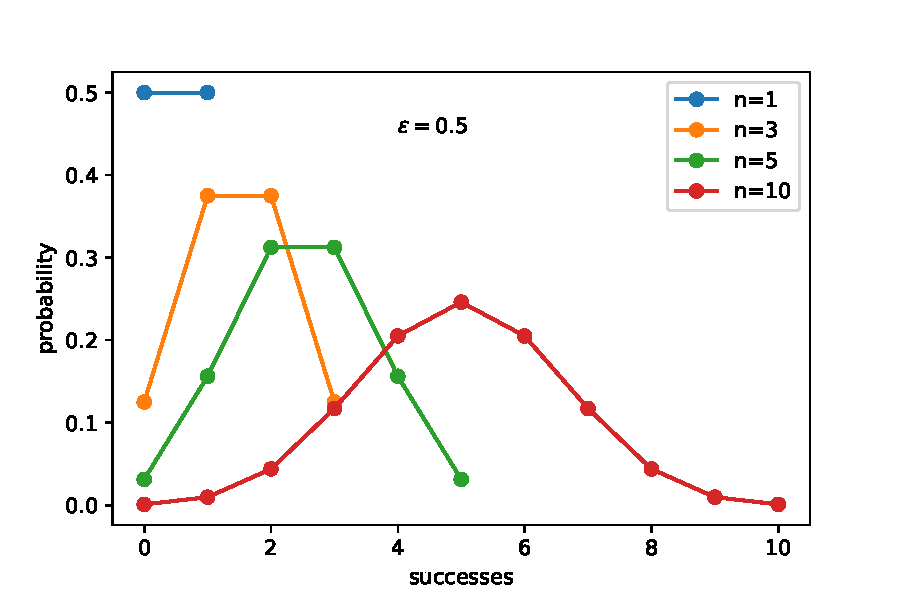
\includegraphics[width=0.47\textwidth]{figs/binom_n.pdf}} &
{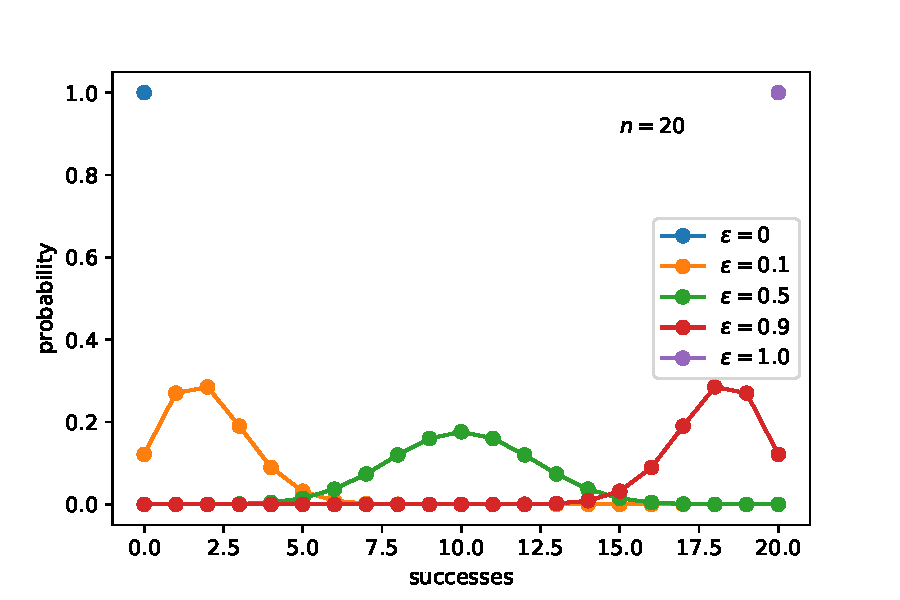
\includegraphics[width=0.47\textwidth]{figs/binom_eps.pdf}} \\
(a) & (b) \\
\end{tabular}
\end{center}
\caption{\label{fig:binom} The binomial distribution for several different values of the parameters (a) $n$ and (b) $\epsilon$.}
\end{figure}

Suppose you repeat a particular process $n$ times, and each time you have the same probability $\epsilon$ of a particular outcome, which, without losing generality, we'll call ``success".  The probability of having exactly $m$ successes after $n$ trials is simply given by:
\begin{displaymath}
P = \sum_i p_i
\end{displaymath}
where $i$ runs over all specific outcomes with $m$ successes and $p_i$ is the probability of each specific outcome.   However, as these specific outcomes all contain exactly $m$ successes, they share the same probability, namely:
\begin{displaymath}
p_i = \epsilon^m (1 - \epsilon)^{n-m}
\end{displaymath}
and so we are left to consider simply the total number of specific outcomes containing $m$ successes.  

The quantity we need is provided by the binomial theorem from mathematics, which states that:
\begin{equation}
\label{eqn:binomt}
(p+q)^n = \sum_{m=0}^{n} \binom{n}{m} \, p^m \, q^{n-m}
\end{equation}
where the binomial coefficients are defined by
\begin{equation}
\label{eqn:binomc}
\binom{n}{m} = \frac{n!}{m! \, (n-m)!}
\end{equation}
and are also often referred to in other contexts as $n$-choose-$m$.  The binomial coefficient simply tells us how many times we can choose $m$ instances of $p$ instead of $q$, from $n$ factors, and so it is precisely the combinatoric factor that we need.

The probability of obtaining $m$ successes after $n$ trials with probability $\epsilon$ is therefore given by:
\begin{equation}
\label{eqn:binom}
P(m; \, n ,\epsilon) = \binom{n}{m} \, \epsilon^m \, (1 - \epsilon)^{n-m}
\end{equation}
which is called the Binomial Distribution.

\subsection{Mean and Variance}

Given a probability distribution, the most urgent questions are generally ``what is the mean value we can expect from this distribution?" and ``how close to the mean value are most of the outcomes?"  The first answer localizes the distribution while the second answer describes its width.

To calculate the mean value in answer to the first question, we simply calculate a weighted average:
\begin{equation}
\braket{m} \equiv \bar{m} \equiv \sum_m m \, P(m) 
\end{equation}
For a continuous probability distribution, we would integrate instead:
\begin{equation}
\braket{x} \equiv \bar{x} \equiv \int x \, P(x) \, dx 
\end{equation}
We usually answer the second question in terms of the variance, $\sigma^2$, of the distribution:
\begin{displaymath}
\sigma^2 \equiv \braket{(x-\bar{x})^2}
\end{displaymath}
Other answers have problems, e.g. $\braket{x-\bar{x}}$ can be zero or nearly so, even for wide distributions, as long as it is symmetric.  You could fix this by calculating $\braket{|x-\bar{x}|}$ but this is generally much harder to calculate, and less useful, than the variance.  For instance, it is left as an exercise to show that:
\begin{equation}
\label{eqn:varhw}
\braket{(x-\bar{x})^2} = \braket{x^2} -\bar{x}^2
\end{equation}
using the fact that $\bar{x}$ is simply a number, and so $\braket{\bar{x}} = \bar{x}$.  We often write this result equivalently as:
\begin{equation}
\label{eqn:variance}
\sigma^2 \equiv \braket{(x-\braket{x})^2} = \braket{x^2} - \braket{x}^2
\end{equation}
Which shows explicitly that we need only calculate $\braket{x}$ and $\braket{x^2}$ in order to determine the variance of a distribution.

\subsection{Mean and Variance of the Binomial Distribution}

The mean value of Binomial Distribution is given by:
\begin{eqnarray*}
\bar{m} &=& \sum_{m=0}^n \; m \, P(m) \\
&=& \sum_{m=0}^n \; m \, \binom{n}{m} \epsilon^m (1-\epsilon)^{n-m} \\
\end{eqnarray*}
which looks rather daunting!  The trick is to use the Binomial Theorem (\ref{eqn:binomt}) and define a function of two independent variables p and q given by:
\begin{displaymath}
f(p,q) = (p+q)^n = \sum_{m=0}^n \binom{n}{m} p^m q^{n-m}
\end{displaymath}
We then calculate:
\begin{displaymath}
\frac{\partial f}{\partial p} = n(p+q)^{n-1} = \sum_{m=0}^n m \binom{n}{m} p^{m-1} q^{n-m} \\
\end{displaymath}
and multiplying by $p$ we have:
\begin{displaymath}
np(p+q)^{n+1} = \sum_{m=0}^n m \binom{n}{m} p^m q^{n-m}
\end{displaymath}
which is true for any $p$ and $q$.  We now substitute the particular values $p=\epsilon$ and $q=1-\epsilon$ and find that:
\begin{displaymath}
n \epsilon = \sum_{m=0}^n m \binom{n}{m} \epsilon^m (1-\epsilon)^{n-m} \equiv \sum_{m=0}^n m P(m) = \bar{m}
\end{displaymath}
So the mean value is given by:
\begin{equation}
\bar{m} = n \epsilon
\end{equation}
or the total number of trials times the probability of success for each trial, a wholly plausible answer.

For the variance, we use a variation of the same trick, this time using the second partial derivative:
\begin{displaymath}
p^2 \cdot \frac{\partial^2 f}{\partial p^2} = n(n-1)p^2(p+q)^{n-2} = \sum_{m=0}^n m (m-1) \binom{n}{m} p^{m} q^{n-m} \\
\end{displaymath}
and again putting $p=\epsilon$ and $q=1-\epsilon$ to find that:
\begin{eqnarray*}
n(n-1)\epsilon^2 &=& \sum_{m=0}^n (m^2 -m) \binom{n}{m} p^{m} q^{n-m} \\[5pt]
&=& \sum_{m=0}^n (m^2 -m) P(m) \\[5pt]
&=& \braket{m^2-m} = \braket{m^2}-\braket{m}
\end{eqnarray*}
and as $\braket{m} = n \epsilon$ we have:
\begin{displaymath}
\braket{m^2} = n(n-1)\epsilon^2 + n \epsilon
\end{displaymath}
And so:
\begin{displaymath}
\sigma^2 = \braket{m^2} - \braket{m}^2 = n(n-1)\epsilon^2 + n \epsilon - n^2\epsilon^2
\end{displaymath}
or simply:
\begin{equation}
\sigma^2 = n \, \epsilon \, (1 - \epsilon)
\end{equation}
Note that if $\epsilon=0$ or $\epsilon=1$, there is only one outcome (all failures or all success) and so the variation is zero.

\subsection{The Poisson Distribution}

\begin{figure}[htbp]
\begin{center}
{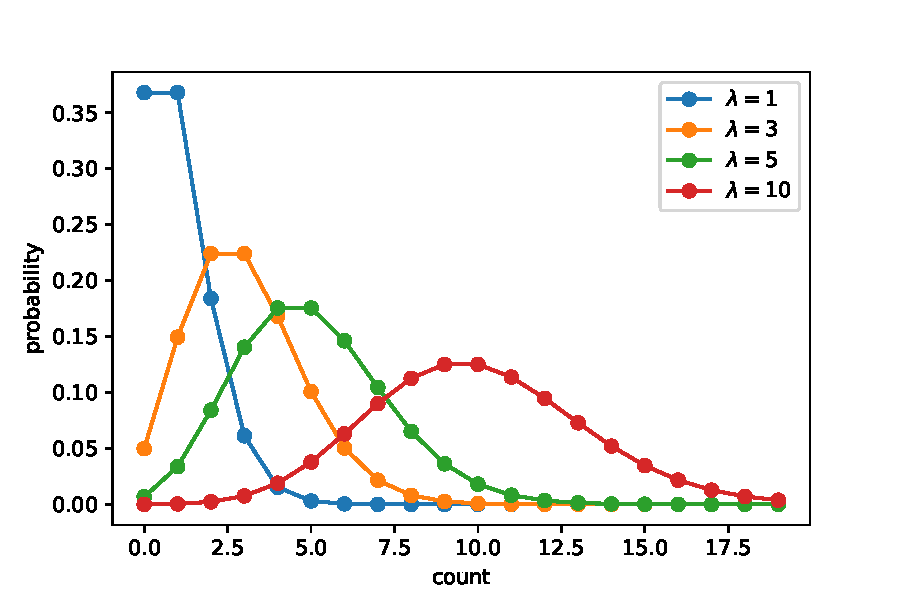
\includegraphics[width=0.45\textwidth]{figs/poisson.pdf}}
\end{center}
\caption{\label{fig:poisson}  The Poisson distribution for several values of parameter $\lambda$.}
\end{figure}


Suppose we have some time interval over which we expect to observe a mean number of events $\lambda$.  The events must be independent of one another:  an event occurring at a particular time cannot affect the time at which the next event occurs.  We divide the time interval over which the $\lambda$ events are expected to occur into into $n$ sub-intervals, each with an equal probability to contain an event.  These intervals will be all the same size if the events are uniformly distributed in time, but if the events are not uniformly distributed, the sub-intervals are simply chosen to ensure the probability is the same in each interval.  Once cast this way, we can interpret this as a binomial distribution, with probability to contain an event, by construction, given by $\epsilon = \lambda / n$:
\begin{eqnarray*}
P(m) &=& \binom{n}{m} \epsilon^m (1-\epsilon)^{n-m} \\[5pt]
  &=& \frac{n!}{m! \, (n-m)!} \; \left( \frac{\lambda}{n} \right)^m \left( 1 - \frac{\lambda}{n}\right)^{n-m} \\[5pt]
  &=& \left( \frac{\lambda^m}{m!} \right) \left(1-\frac{\lambda}{n} \right)^n \left[ \frac{n!}{(n-m)!} \cdot \frac{1}{n^m}\right]_1 \left[ \left( 1 - \frac{\lambda}{n}\right)^{-m}\right]_2
\end{eqnarray*}
We obtain the Poisson distribution by considering the limit that  $n \to \infty$.   It is left as an exercise to show that both $[\dots]_1 \to 1$ and $[\dots]_2 \to 1$ as $n \to \infty$.  Recalling that
\begin{displaymath}
\lim_{n \to \infty} \left(1 - \frac{\lambda}{n} \right)^n = e^{-\lambda}
\end{displaymath}
we obtain the Poisson distribution, the probability for observing $m$ events for a mean of $\lambda$:
\begin{equation}
\label{eqn:poisson}
P(m\; ; \; \lambda) = \frac{\lambda^m}{m!} \, e^{-\lambda}
\end{equation}
Notice that there is no longer a parameter $n$, since we took $n \to \infty$, and so $m$ now ranges from 0 to $\infty$.

\subsection{Mean and Variance of The Poisson Distribution}

The mean of the Poisson distribution is given by:
\begin{eqnarray*}
\bar{m} &=& \sum_{m \geq 0} \; m \, P(m) \\
&=& \sum_{m \geq 0} \; m \, \frac{\lambda^m}{m!} \, e^{-\lambda}\\
\end{eqnarray*}
Since the first term ($m=0$) is zero, we have:
\begin{eqnarray}
\bar{m} &=& e^{-\lambda} \sum_{m \geq 1} \; \frac{\lambda^m}{(m-1)!} \notag \\
             &=& \lambda e^{-\lambda} \sum_{m \geq 1} \; \frac{\lambda^{m-1}}{(m-1)!} \notag \\
             &=& \lambda e^{-\lambda} \sum_{n \geq 0} \; \frac{\lambda^{n}}{n!} \notag \\
             &=& \lambda e^{-\lambda} e^\lambda \notag \\
\bar{m}  &=& \lambda
\end{eqnarray}
which should come as no surprise, as the assumption in the derivation was the that mean number of events was $\lambda$.

For the variance, we use a similar manipulation to calculate:
\begin{eqnarray*}
\braket{m^2} &=& \sum_{m \geq 0} \; m^2 \, P(m) \\
&=& \sum_{m \geq 0} \; m^2 \, \frac{\lambda^m}{m!} \, e^{-\lambda}\\
&=& \lambda \sum_{m \geq 1} \; m \, \frac{\lambda^{m-1}}{(m-1)!} \, e^{-\lambda}\\
&=& \lambda \sum_{n \geq 0} \; (n+1) \, \frac{\lambda^{n}}{(n)!} \, e^{-\lambda}\\
&=& \lambda \braket{m+1} = \lambda \, (\lambda+1)
\end{eqnarray*}
And so:
\begin{eqnarray}
\sigma^2 &=& \braket{m^2} - \braket{m}^2 \notag \\
&=& \lambda \, (\lambda+1) - \lambda^2 \notag \\
\sigma^2 &=& \lambda. 
\end{eqnarray}
That is, the variance of a Poisson distribution is simply the mean.

\subsection{The Gaussian Distribution}

\begin{figure}[htbp]
\begin{center}
{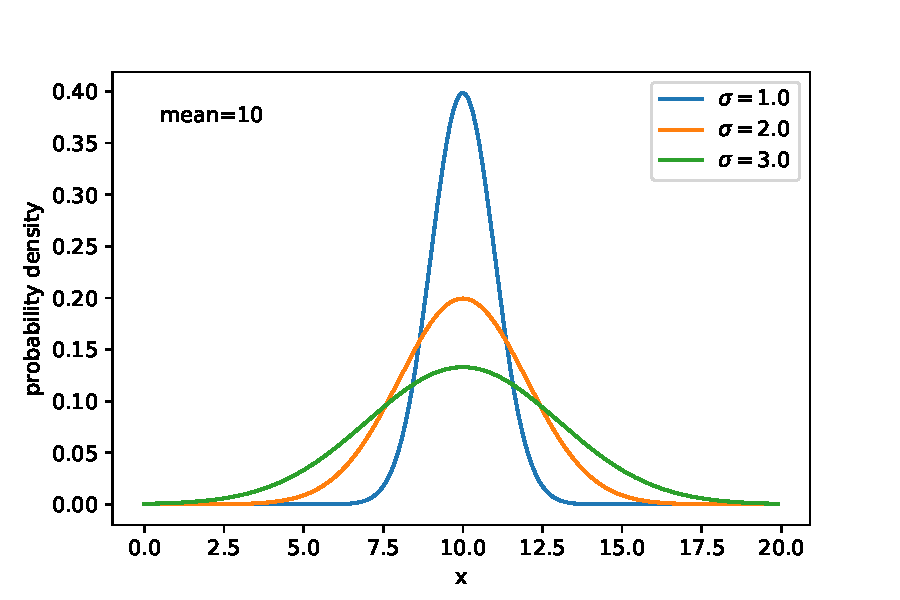
\includegraphics[width=0.45\textwidth]{figs/gaussian.pdf}}
\end{center}
\caption{\label{fig:poisson}  The Gaussian distribution for a mean of 10 and several values of parameter $\sigma$.}
\end{figure}

Next, we consider the Poisson Distribution in the limit $\lambda \to \infty$.  In this case, we can apply the Stirling Approximation:
\begin{displaymath}
\lim_{n \to \infty} n! = \sqrt{2 \pi n} \; e^{-n} \; n^n
\end{displaymath}
to the Poisson distribution as follows:
\begin{eqnarray*}
P(m) &=& \frac{\lambda^m}{m!} \, e^{-\lambda} \\[5pt]
 &\to& \frac{\lambda^m e^{-\lambda}}{\sqrt{2 \pi m} \; e^{-m} \; m^m} \\[5pt]
 &=& \frac{e^{m-\lambda}}{\sqrt{2\pi\lambda}} \left( \frac{\lambda}{m}\right)^{m+\frac{1}{2}}\\
\end{eqnarray*}
Now we consider a new variable $\delta$, defined by
\begin{displaymath}
\delta \equiv \frac{m-\lambda}{\lambda}
\end{displaymath}
which measures the difference between the observed number of events $m$ and the mean of the distribution, as a fraction of the mean.  Intuitively, the function is getting very narrow, and so we expect this to be a small quantity, but let's check this.  First we have:
\begin{displaymath}
\braket{\delta} = \frac{\braket{m}- \lambda}{\lambda} = \frac{\lambda - \lambda}{\lambda} = 0
\end{displaymath}
but also:
\begin{displaymath}
\braket{\delta^2} = \frac{\braket{(m-\lambda)^2}}{\lambda^2} = \frac{\lambda}{\lambda^2} = \frac{1}{\lambda}
\end{displaymath}
where we have used the fact that the variance is given by $\braket{(m-\lambda)^2} = \lambda$, and so as $\lambda \to \infty $ we have
\begin{displaymath}
\braket{\delta^2} \to 0
\end{displaymath}
So we can write:
\begin{equation} \label{eqn:mdef}
m = \lambda (1 + \delta)
\end{equation}
where we expect the approximation $\delta \to 0$ to hold as long as we require $\lambda \to \infty$.  So now we can write the distribution in terms of the small quantity $\delta$ and the large quantity $\lambda$ as:
\begin{eqnarray}
\label{eqn:pdelt}
P(\delta) &=& \frac{e^{\lambda\delta}}{\sqrt{2\pi\lambda}} \left( \frac{\lambda}{\lambda (1+\delta)} \right)^{\lambda(1+\delta)+\frac{1}{2}} \notag \\[5pt]
 &=& \frac{e^{\lambda\delta}}{\sqrt{2\pi\lambda}} \cdot \frac{1}{X}
\end{eqnarray}
where we define the quantity:
\begin{displaymath}
X = (1+\delta)^{\lambda(1+\delta)+\frac{1}{2}}
\end{displaymath}
which can be approximated as follows:
\begin{eqnarray*}
\ln X &=& \left( \lambda (1+\delta) + \frac{1}{2} \right) \cdot \ln(1+\delta) \\[5pt]
&=& \left( \lambda (1+\delta) + \frac{1}{2} \right) \cdot \left( \delta - \frac{\delta^2}{2} + \mathcal{O}(\delta^3)\right) \\[5pt]
\frac{\ln X}{\lambda}&=& \left( 1+\delta + \frac{1}{2\lambda} \right) \cdot \left( \delta - \frac{\delta^2}{2} + \mathcal{O}(\delta^3)\right) \\[5pt]
&=& \left( 1+\delta + \mathcal{O}\left(\delta^2\right) \right) \cdot \left( \delta - \frac{\delta^2}{2} + \mathcal{O}(\delta^3)\right) \\[5pt]
&=& \delta + \frac{\delta^2}{2}+ \mathcal{O}(\delta^3),
\end{eqnarray*}
where in the second to last step we used $\mathcal{O}\left(\frac{1}{\lambda}\right) \sim \mathcal{O}\left(\delta^2\right)$.  Neglecting the small quantities, we can approximate
\begin{displaymath}
X = \exp\left( \lambda\delta + \lambda\frac{\delta^2}{2} \right) 
\end{displaymath}
which, when plugged backed into Equation~\ref{eqn:pdelt} yields:
\begin{eqnarray}
\label{eqn:almost}
P(\delta) &=& \frac{e^{\lambda\delta}}{\sqrt{2\pi\lambda}} \cdot \frac{1}{\exp\left( \lambda\delta + \lambda\frac{\delta^2}{2} \right)} \notag \\[5pt]
&=& \frac{1}{\sqrt{2\pi\lambda}} \cdot \exp\left( -\lambda \frac{\delta^2}{2}\right)
\end{eqnarray}
Now notice that Equation~\ref{eqn:mdef} implies that $m$ is quite large, and so may now be treated as a continuous variable, which we will rename $x$ (since $m$ looks like an integer value), hence we have:
\begin{displaymath}
\delta \equiv \frac{m - \lambda}{\lambda} = \frac{x - \lambda}{\lambda}
\end{displaymath}
and likewise we know that the variance of the original Poisson distribution is given by $\sigma^2 = \lambda$, and so we can rewrite Equation~\ref{eqn:almost}
in the (hopefully) more familiar form:
\begin{equation}
\label{eqn:gaussian}
P(x) = \frac{1}{\sqrt{2\pi} \sigma} \cdot \exp\left( - \frac{(x - \lambda)^2}{2 \sigma^2}\right)
\end{equation}
Which is a Gaussian distribution with mean value $\lambda$ and variance $\sigma^2$.  The proof that these quantities are indeed the mean and the variance is left as an exercise.

\subsection{Continuous versus Discrete Distributions}

The Binomial and Poisson distributions are not continuous functions:  they describe the probability of outcomes which are integer quantities.   The Poisson probability for having 2.31 events is either undefined or taken to be zero.  The value of the Binomial and Poisson distribution function at a particular integer value is simply the probability of that particular outcome.  To determine the probability that an outcome is within a range of integers, say $m_1$ to $m_2$ the probability distribution function is simply added:
\begin{displaymath}
P = \sum_{m=m_1}^{m_2} P(m).
\end{displaymath}

The Gaussian distribution is a continuous function: it describes the probability density function of a particular value of $x$.  The probability of any particular outcome, say $x=1.24323$, is vanishing small.  But the probability that the value lies within a range of values can be non-zero, and is determined by integrating:
\begin{displaymath}
P = \int_{x_{\rm min}}^{x_{\rm max}} P(x) \, dx
\end{displaymath}
The probability distribution function is normalized so that:
\begin{displaymath}
\int_{-\infty}^{+\infty} P(x) \, dx = 1
\end{displaymath}
To determine the mean value of a function $f(x)$ we likewise integrate:
\begin{displaymath}
\braket{f(x)} \equiv \int_{-\infty}^{+\infty} f(x) P(x) \, dx = 1
\end{displaymath}
In particular the mean value of $x$ is:
\begin{displaymath}
\braket{x} \equiv \int_{-\infty}^{+\infty} x P(x) \, dx = 1
\end{displaymath}
and:
\begin{displaymath}
\braket{x^2} \equiv \int_{-\infty}^{+\infty} x^2 P(x) \, dx = 1
\end{displaymath}
with:
\begin{displaymath}
\sigma^2 = \braket{x^2} -\braket{x}^2.
\end{displaymath}

The Gaussian distribution is a probability density function (PDF), because it reports a probability density.  A discrete probability distribution is sometimes referred to as probability mass function (PMF), to draw upon an analogy with physical mass and density.

\subsection{Histograms in Scientific Python}

\begin{figure}[htbp]
\begin{center}
\begin{tabular}{cc}
{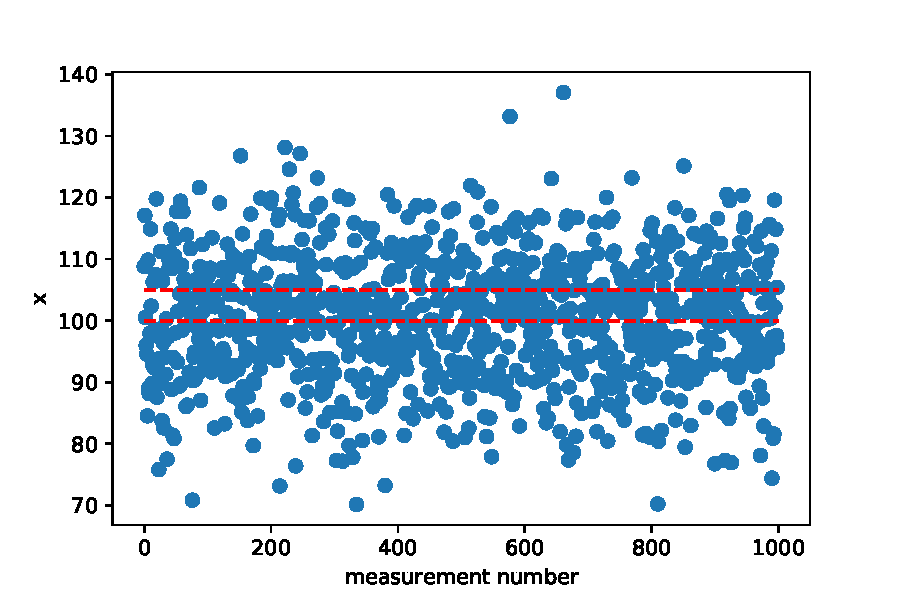
\includegraphics[width=0.45\textwidth]{figs/raw.pdf}} &
{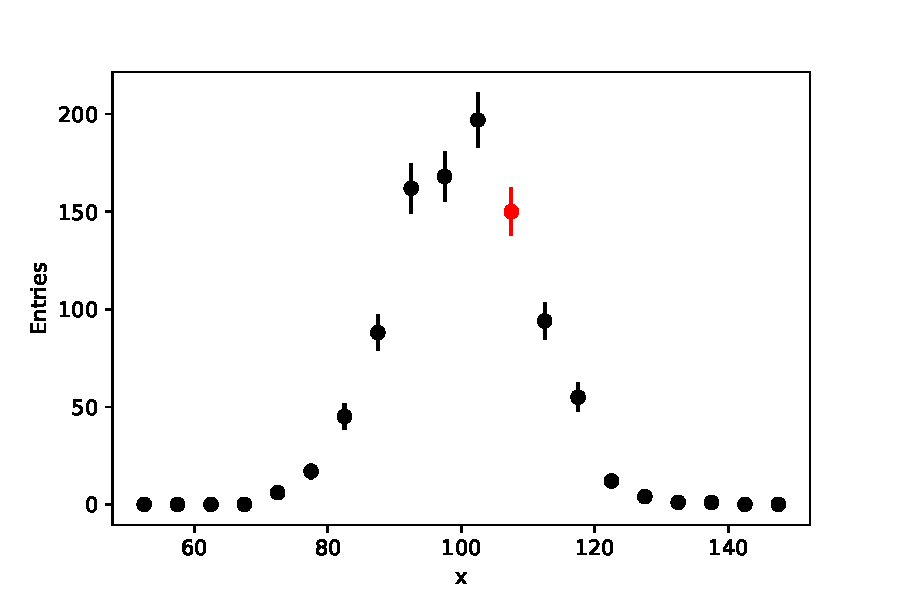
\includegraphics[width=0.45\textwidth]{figs/histeg.pdf}} \\
(a) & (b) \\
\end{tabular}
\end{center}
\caption{\label{fig:histeg} The 1000 measurements of variable $x$ in (a) are used to produce the histogram in (b).  The red data point in (b) is the count of the number of entries in range indicated by the red dashed lines in (a).}
\end{figure}

Suppose a particular variable $x$ is measured 1000 times.  One way to visualize the collected data is shown in Fig.~\ref{fig:histeg}a, which simply plots each measurement value above the measurement number (from 0 to 1000).  In this example, the number of measurements that occur within the range from $x=100$ to $x=105$ is 181.  This count is plotted as the red data point in Fig.~\ref{fig:histeg}b, 181 entries located above $x=102.5$, the center of the range.  If we repeat this exercise across a number or ranges, the resulting plot in Fig.~\ref{fig:histeg}b is called a histogram.  A histogram reports the number of entries that occur within each of a sequence of consecutive ranges of $x$-values.  Each range considered is called a histogram  bin, and the choice of which bins to use is at the discretion of the analyzer.

The content of each bin is a single number, a count, and is therefore subject to the Poisson distribution.
We can estimate the mean of the Poisson distribution by the measured value, so that $\lambda = N$.
For the Poisson distribution, the variance $\sigma^2 = \lambda$, and so $\sigma = \sqrt{N}$.  It is customary to draw a line of size $\sqrt{N}$ when plotting a histogram value $N$. This is an example of an error bar, which indicates how well our measurement has determined a particular value.

\begin{figure}[htbp]
\begin{center}
{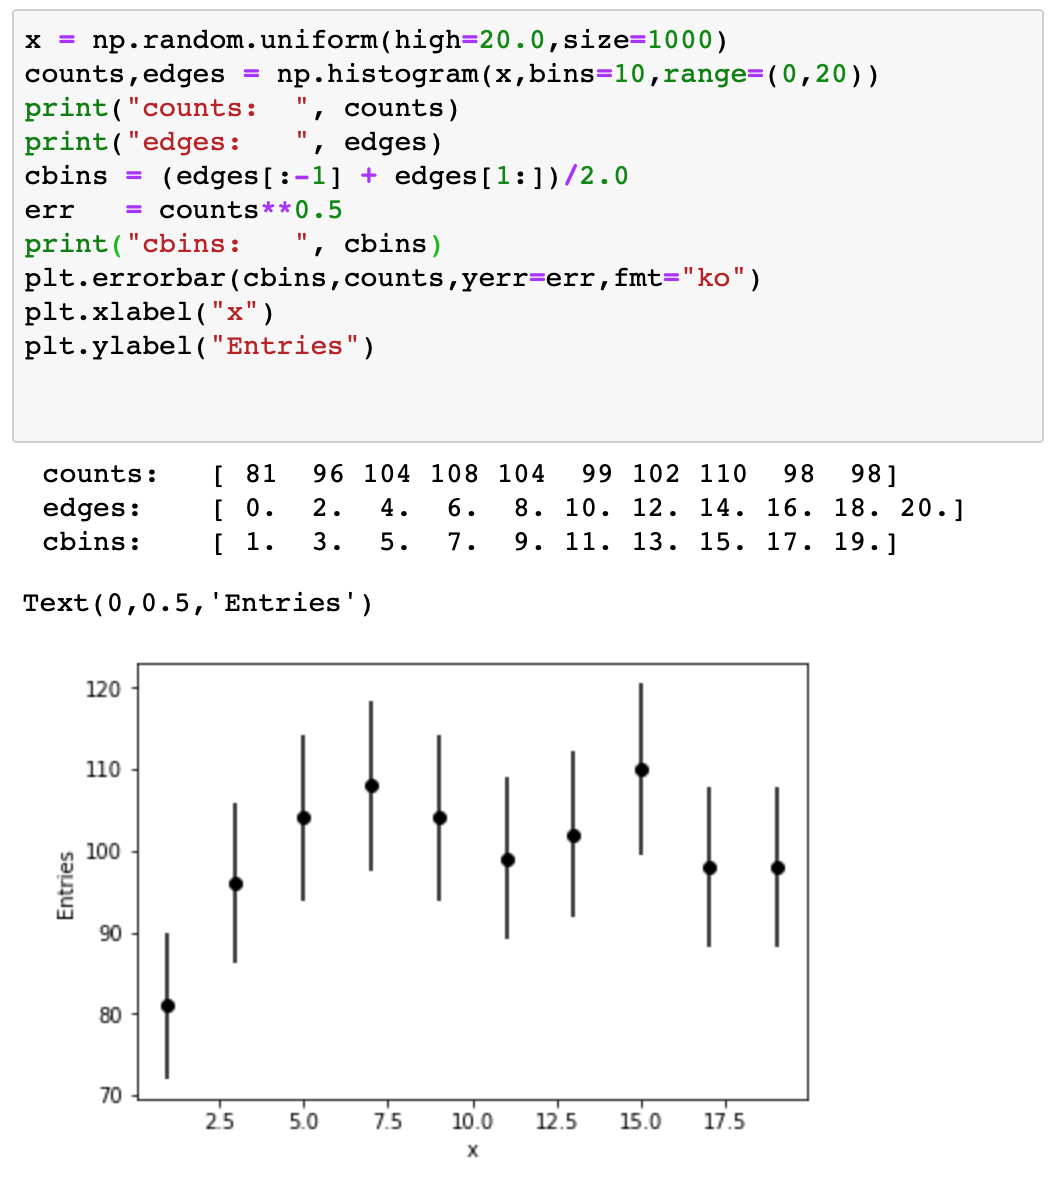
\includegraphics[width=0.85\textwidth]{figs/makehisteg.png}} 
\end{center}
\caption{\label{fig:makehisteg} Example producing a histogram in Scientific Python.}
\end{figure}

An example producing a histogram in Scientific Python is shown in Fig.~\ref{fig:makehisteg}.
The data to plot is simply a sequence of 1000 values randomly and uniformly chosen in the range $[0,20]$:
\begin{verbatim}
x = np.random.uniform(high=20.0,size=1000)
\end{verbatim}
To create a histogram from these 1000 values, we use the {\tt np.histogram} function:
\begin{verbatim}
counts,edges = np.histogram(x,bins=10,range=(0,20))
\end{verbatim}
where we have specified 10 bins, uniformly covering the range from 0 to 20.  The 
function returns to arrays, which we save as {\tt counts} and {\tt edges}.  The {\tt counts} array contains the bin contents, the count of the number of values in each bin: 
\begin{verbatim}
counts:   [ 92  82 123  96  85 106 105  99  99 113]
\end{verbatim}
The edges array contains the edges of the bins:
\begin{verbatim}
edges:    [ 0.  2.  4.  6.  8. 10. 12. 14. 16. 18. 20.]
\end{verbatim}
You'll notice that 10 consecutive bins have 11 edges.  For plotting continuous data, one choice is to plot the contents at the center of each bin:
\begin{verbatim}
cbins = (edges[:-1] + edges[1:])/2.0
\end{verbatim}
the two slices {\tt edges[:-1]} and {\tt edges[1:]} are all but the last and all but the first.  The average of the two is the center of each bin:
\begin{verbatim}
cbins:    [ 1.  3.  5.  7.  9. 11. 13. 15. 17. 19.]
\end{verbatim}
The error bar values are chosen as the square root of the bin values:
\begin{verbatim}
err   = counts**0.5
\end{verbatim}
The histogram is plotted using the {\tt plt.errorbar} function:
\begin{verbatim}
plt.errorbar(cbins,counts,yerr=err,fmt="ko")
\end{verbatim}
which plots the bin contents {\tt counts} at the bin center values {\tt cbins} using the square root error bars in the array {\tt err}, using the format {\tt "ko"} for black circles.

\subsection{Comparing a Histogram to a Probability Distribution Function}

Our theoretical models often predict a PDF for some observable variable $x$.  As experimentalists, we are often therefore concerned with the question as to whether our collected data for an observable $x$ is consistent with the theoretical PDF.  A visual approach to answering this question is to plot the data in a histogram, and to draw the PDF as a curve normalized to the histogram.

To predict the number of events in a bin with edges $x_{\rm lower}$ and $x_{\rm upper}$, in principle we need to integrate the PDF and normalize to the number of experiments:
\begin{displaymath}
N_{\rm pred} = N_{\rm meas} \int^{x_{\rm upper}}_{x_{\rm lower}} p(x) \, dx
\end{displaymath}
In practice, we generally choose the bin sizes small enough that the PDF is approximately constant during the entire bin, and in this case, the prediction can be taken as:
\begin{displaymath}
N_{\rm pred} = N_{\rm meas} \; \Delta x \; p(x)
\end{displaymath}
where $\Delta x$ is the width of each bin.  This scale factor $N_{\rm meas} \; \Delta x$ allows us to compare a continuous function to data collected in discrete bins, as shown in Fig.~\ref{fig:histpdf}.

\begin{figure}[htbp]
\begin{center}
{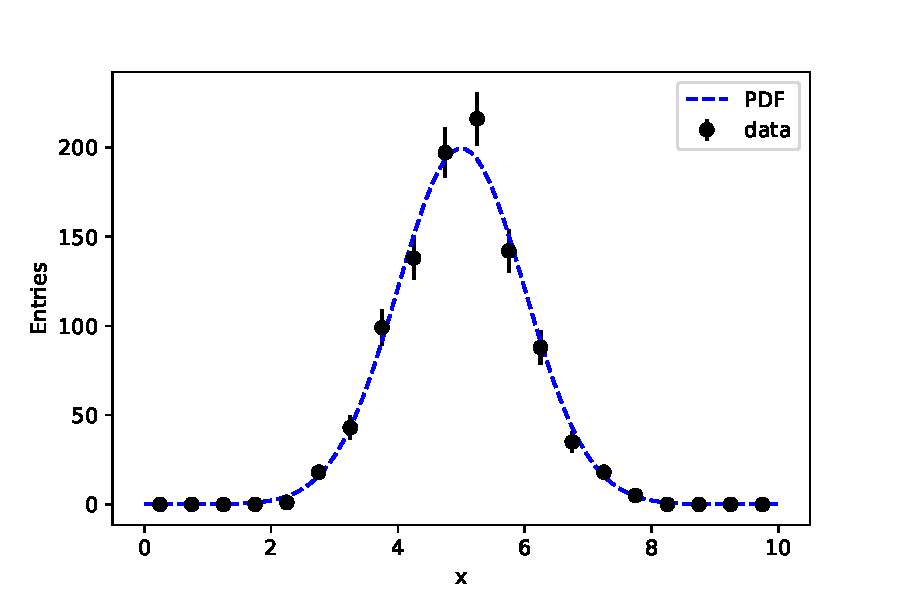
\includegraphics[width=0.65\textwidth]{figs/compare.pdf}}
\end{center}
\caption{\label{fig:histpdf} The Gaussian PDF scaled to compare to data from a Gaussian distribution.
In this case, there are 1000 total entries in the histogram and the bin size is 0.5, for a scale factor of 500.
}
\end{figure}

\newpage
\subsection{Homework Exercises for Distributions}

\noindent
{\bf Problem 1:} Show that the Binomial distribution, $P(m)$, in Equation~\ref{eqn:binom} is properly normalized:
\begin{displaymath}
\sum_{m=0}^n P(m) = 1
\end{displaymath}
as a consequence of the Binomial Theorem (Equation~\ref{eqn:binomt}).

\vskip 1cm
\noindent
{\bf Problem 2:} Show that Equation~\ref{eqn:varhw} is correct.

\vskip 1cm
\noindent
{\bf Problem 3:} Show that the Poisson distribution, $P(m)$, in Equation~\ref{eqn:poisson} is properly normalized:
\begin{displaymath}
\sum_{m \geq 0} P(m) = 1.
\end{displaymath}
Hint: recall the Taylor series expansion for $e^\lambda$.

\vskip 1cm
\noindent
{\bf Problem 4:} Show that the Gaussian distribution, $P(x)$, in Equation~\ref{eqn:gaussian} is properly normalized:
\begin{displaymath}
\int_{-\infty}^{\infty} P(x) dx = 1.
\end{displaymath}

\vskip 1cm
\noindent
{\bf Problem 5:} Show that the mean of the Gaussian distribution has been correctly identified in Equation~\ref{eqn:gaussian}.  That is, show explicitly that:
\begin{displaymath}
\int_{-\infty}^{\infty} x P(x) dx = \lambda 
\end{displaymath}

\vskip 1cm
\noindent
{\bf Problem 6:} Show that the variance of the Gaussian distribution has been correctly identified in Equation~\ref{eqn:gaussian}.  That is, show explicitly that:
\begin{displaymath}
\int_{-\infty}^{\infty} x^2 P(x) dx = \sigma^2 
\end{displaymath}
when we take $\lambda=0$ (which is equivalent to simply changing variables $y=x-\lambda$.)
   
%\section{Challenges (Not Assigned)}
%
%\noindent
%{\bf Problem 1:} Prove by induction the formula for the binomial coefficients in (Equation~\ref{eqn:binomc}).

\end{document}

\newpage

\section{Statistical Uncertainties}

\subsection{Precision versus Accuracy}

\ldots
\subsection{Importance of the Gaussian Distribution}

\subsection{Reporting Experimental Uncertainties}

A scientific measurement is meaningless without an associated uncertainty.  The convention is to report only one significant digit worth of uncertainty (or two if the first digit is a 1 or 2).  So we don't report $x = 1.234 \pm 0.303~\rm{m}$, but instead would report $x= 1.2 \pm 0.3~\rm{m}$ or $t = 4.76 \pm 0.13~\rm{s}$. 

The uncertainty is intended to indicate how close the true value for measured quantities is to the best estimate.  The Central Limit Theorem informs us that the sum of a large number of random variables approaches a Gaussian distribution.  Since experimental measurements are often repeated many times, and the sources of noise causing the measurement to differ from the true value are numerous, most often the experimental uncertainties can be treated as coming from a Gaussian distribution.  That is to say that the true value of the measured quantity is assumed to be described by a Gaussian distribution with mean value at the best estimated value and with $\sigma$ given by the reported uncertainty.

\subsection{The Error Function}

Suppose we measure the speed of light in vacuum to be:
\begin{displaymath}
3.3 \pm 0.2 \times 10^8~{\rm m}/{\rm s}^2
\end{displaymath}
How consistent is this with the generally accepted value:
\begin{displaymath}
3.0 \times 10^8~{\rm m}/{\rm s}^2
\end{displaymath}
where we have omitted the uncertainty here because it is much smaller than our uncertainty!   The interpretation of the uncertainty as the $\sigma$ of a Gaussian distribution allows us to give quite precise answers.  To begin we might say that it is consistent within:
\begin{displaymath}
\frac{3.3 - 3.0}{0.2} = 1.5 \; \sigma.
\end{displaymath}
but we can also ask, what is the probability enclosed in $1.5 \sigma$.  To  answer this question, we use the error function:
\begin{displaymath}
{\rm erf}(x) = \frac{1}{\sqrt{\pi}} \int^x_{-x} \exp\left(-t^2 \right) dt
\end{displaymath}
which is simply the integral from $-x$ to $x$ of a Gaussian with $\sigma = 1/sqrt{2}$.  So if we want to calculate the probability contained in $n~\rm sigma$ we would calculate:
\begin{displaymath}
 {\rm erf}(n \cdot \frac{1}{\sqrt{2}})
\end{displaymath}
which is tabulated in Table~\ref{tbl:erf}.\\

\begin{table}[thb]
\begin{center}
\begin{tabular}{lll}
interval & error function & integrated probability \\ 
\hline
$\pm1 \sigma$ & ${\rm erf}\left( \frac{1}{\sqrt{2}} \right)$ & 68.3\% \\
$\pm2 \sigma$ & ${\rm erf}\left( \frac{2}{\sqrt{2}} \right)$ & 95.4\% \\
$\pm3 \sigma$ & ${\rm erf}\left( \frac{3}{\sqrt{2}} \right)$ & 98.5\% \\
$\pm4 \sigma$ & ${\rm erf}\left( \frac{4}{\sqrt{2}} \right)$ & 99.5\% \\
$\pm5 \sigma$ & ${\rm erf}\left( \frac{5}{\sqrt{2}} \right)$ & 99.8\% \\ 
\end{tabular}
\caption{\label{tbl:erf} The integrated probability for a Gaussian distribution within the stated bounds.} 
\end{center}
\end{table}

\subsection{Mean and Variance of a Sum}

So far we've been calculating expectation values of functions of one random variable: 
\begin{displaymath}
\braket{f(x)} = \int f(x) \; P(x) \; dx
\end{displaymath}
but this easily generalizes to two or more random variables:
\begin{displaymath}
\braket{f(x,y)} = \int \int f(x,y) \; P(x,y) dx \, dy 
\end{displaymath}
If the random variables are independent, then we have $P(x,y) = P(x) \, P(y)$ and so
\begin{displaymath}
\braket{f(x,y)} = \int f(x,y) \; P(x) \, P(y) \; dx \, dy
\end{displaymath}
And also we have
\begin{eqnarray*}
\braket{f(x)+g(y)} &=& \int \int dx \, dy \; P(x) \, P(y) \;\; (f(x) + g(y)) \\
&=& \left(\int P(y) \; dy \right) \cdot \left( \int P(x) \; f(x) \; dx  \right) 
+ \left(\int P(x) \; dx \right) \cdot \left( \int P(y) \; f(y) \; dy  \right)\\
&=& 1 \cdot \int P(x) \; f(x) \; dx  + 1 \; \cdot \int P(y) \; f(y) \; dy \\
\end{eqnarray*}
which we can write much more simply as:
\begin{displaymath}
\braket{f(x)+g(y)} = \braket{f(x)}+\braket{g(y)}
\end{displaymath}
revealing the power of the expectation value notation for tackling independent random variables.  In the homework you will show that similarly:
\begin{equation}
\braket{f(x) \cdot g(y)} = \braket{f(x)} \cdot \braket{g(y)} \label{eqn:expprod}
\end{equation}
We can therefore conclude that the mean of a sum of two random variables:
\begin{displaymath}
\braket{x + y} = \braket{x} + \braket{y} 
\end{displaymath}
is just the sum of the mean.  Supposing that $\braket{x} = \braket{y} = 0$ we also have:
\begin{eqnarray*}
\braket{(x + y)^2} &=& \braket{x^2 + 2*x*y + y^2} \\
&=& \braket{x^2} + 2*\braket{x}*\braket{y} + \braket{y^2} \\
&=& \braket{x^2} + \braket{y^2} \\
\end{eqnarray*}
In the exercises you will show using expectation values that the variance of the sum of two independent random variables is just the sum of their variances:
\begin{displaymath}
\sigma^2(x+y) = \sigma^2_x + \sigma^2_y
\end{displaymath}

\subsection{Uncertainties Add in Quadrature}

In the previous section, we discussed that the variance of the sum of two random variables drawn from any distribution is just the sum of their variances:
\begin{displaymath}
\sigma^2(x+y) = \sigma^2_x + \sigma^2_y
\end{displaymath}
This is a quite general result.  In the context of experimental uncertainties, we consider experimental measurements to be drawn from a Gaussian distribution and the square-root of the variance ($\sigma$) is called the uncertainty.

If we calculate the sum $s$ of two independent measurements $x$ and $y$ with uncertainties $\sigma_x$ and $\sigma_y$, it's clear that the variance of the sum will be simply $\sigma^2_x + \sigma^2_y$.  If the resulting distribution of $x+y$ is a Gaussian distribution, as seems probable due to the Central Limit Theorem, then the uncertainties simply add in quadrature:
\begin{displaymath}
\sigma_{x+y} = \sqrt{\sigma^2_x + \sigma^2_y}.
\end{displaymath}

Let's show explicitly that this is the case.  If we wish to know the probability that two random variables $x$ and $y$ add to some particular value $u = x + y$, we simply integrate the total probability of $x$ and $y$ subject to the requirement $u = x + y$:
\begin{eqnarray*}
P(u) &=& \int dx \int dy \; P_x(x) \, P_y(y) \, \delta\left(u-(x+y)\right) \\
        &=& \int dx \; P_x(x) \, P_y(u-x)
\end{eqnarray*}
If we make the (very often valid) assumption that $x$ and $y$ are Gaussian distributed, and, for simplicity, assume that the mean values are zero (or simply change coordinates), so that we have:
\begin{eqnarray*}
P_x(x) &=& \frac{1}{\sqrt{2\pi} a} \exp\left( -\frac{x^2}{2a^2} \right) \\
P_y(y) &=& \frac{1}{\sqrt{2\pi} a} \exp\left( -\frac{y^2}{2b^2} \right) 
\end{eqnarray*}
And so the mean value probability distribution function for $u$ is now:
\begin{eqnarray*}
P(u) &=& \frac{1}{2\pi a b} \int dx \; \exp\left( -\frac{x^2}{2a^2}\right) \exp\left( -\frac{(u-x)^2}{2b^2}\right) \\
&=& \frac{1}{2\pi a b} \int dx \; \exp \left( -\frac{a^2+b^2}{2a^2b^2} \, \left\{ x^2 - \frac{2a^2}{a^2+b^2}ux + \frac{a^2}{a^2+b^2}u^2\right\}_1 \right) 
\end{eqnarray*}
We deal with the term in brackets ($\{\}_1$) by completing the square.  Simply note that
\begin{equation}
\left(x-\frac{a^2}{a^2+b^2}u\right)^2 = x^2-\frac{2a^2}{a^2+b^2}ux + \frac{a^4}{(a^2+b^2)^2}u^2
\end{equation}
reproduces the first and second terms, so we can replace:
\begin{equation}
x^2-\frac{2a^2}{a^2+b^2}ux  = \left(x-\frac{a^2}{a^2+b^2}u\right)^2 -  \frac{a^4}{(a^2+b^2)^2}u^2
\end{equation}
to obtain:
\begin{eqnarray*}
\{\}_1 &=& \left(x-\frac{a^2}{a^2+b^2}u\right)^2 -  \frac{a^4}{(a^2+b^2)^2}u^2 + \frac{a^2}{a^2+b^2}u^2\\
&=& \left(x-\frac{a^2}{a^2+b^2}u\right)^2 + \frac{a^2b^2}{(a^2+b^2)^2}u^2\\
\end{eqnarray*}
and substituting back into the original expression we obtain:
\begin{eqnarray*}
P(u) &=& \frac{1}{2\pi a b} \left\{ \int_{-\infty}^{+\infty} dx \;  \exp \left( -\frac{a^2+b^2}{2a^2b^2} \, \left(x-\frac{a^2}{a^2+b^2}u\right)^2 \right) \right\}_2
\exp \left( -\frac{1}{2} \frac{u^2}{a^2+b^2} \right)
\end{eqnarray*}
making a substitution of variables ($u$ is constant during the integration):
\begin{equation*}
y = x-\frac{a^2}{a^2+b^2}u
\end{equation*}
the definite integral in brackets yields:
\begin{equation}
\{\}_2 = \sqrt(2 \pi) \frac{a b}{\sqrt{a^2+b^2}}
\end{equation}
and we have at last:
\begin{eqnarray*}
P(u) &=& \frac{1}{\sqrt{2\pi} \sqrt{a^2+b^2}}  \exp \left( -\frac{1}{2} \frac{u^2}{a^2+b^2} \right)
\end{eqnarray*}
which is a Gaussian distribution with variance:
\begin{eqnarray*}
\sigma^2 = a^2 + b^2,
\end{eqnarray*}
that is, uncertainties add in quadrature.

\subsection{Handling Constants}

When adding a known constant to a measured quantity:
\begin{equation*}
y = x + C
\end{equation*}
we can consider the constant to have uncertainty $\sigma=0$.  And therefore, from the addition in quadrature rule:
\begin{equation*}
\sigma_y = \sigma_x
\end{equation*}

If we multiply a measured quantity by a known constant 
\begin{equation*}
y = k x 
\end{equation*}
we consider that:
\begin{displaymath}
dx \frac{1}{\sqrt{2\pi} \sigma} \exp\left(-\frac{(x-\mu)^2}{2\sigma^2}\right) = d(kx) \frac{1}{\sqrt{2\pi} k\sigma} \exp\left(-\frac{(kx-k\mu)^2}{2(k\sigma)^2}\right)
\end{displaymath}
and conclude that:
\begin{equation*}
\sigma_y = k \sigma_x
\end{equation*}

\subsection{General Propagation of Uncertainties}
We are now ready to handle propagation of uncertainties for a general function.  Suppose we measure $x = x_0 \pm \sigma_x$ and $y = y_0 \pm \sigma_y$ and we wish to know the resulting uncertainty on the calculated quantity $f(x,y)$.

Now we Taylor expand the function about the measured values $x_0$ and $y_0$:
\begin{equation*}
f(x,y) = f(x_0+\Delta x,y_0 + \Delta y) \sim f(x_0,y_0) + \left.\frac{df}{dx}\right|_{x_0,y_0} \Delta x + \left.\frac{df}{dy}\right|_{x_0,y_0} \Delta y 
\end{equation*}
We note that 
\begin{eqnarray*}
\Delta x \equiv x - x_0 \\
\Delta y \equiv y - y_0 \\
\end{eqnarray*}
where we can consider $x_0$ and $y_0$ to be precisely known constants that happen to coincide with our best measured value of $x$ and $y$.  In this case, our measurement amounts to:
\begin{eqnarray*}
\Delta x &=& 0 \pm \sigma_x\\
\Delta y &=& 0 \pm \sigma_y\\
\end{eqnarray*}
and our uncertainties are associated with $\Delta x$ and $\Delta y$, not the ``constants" $x_0$ and $y_0$.

Turning back to the Taylor expansion, we see now that:
\begin{equation*}
f(x,y) \sim A + B \Delta x + C \Delta y 
\end{equation*}
where the constants are:
\begin{eqnarray*}
A  &=& f(x_0,y_0)\\
B  &=& \left.\frac{df}{dx}\right|_{x_0,y_0}\\
C  &=& \left.\frac{df}{dy}\right|_{x_0,y_0}\\
\end{eqnarray*}
We know how to propagate uncertainties in this case, which involves scaling, adding in quadrature, and adding a constant:
\begin{equation*}
\sigma_f^2 =   B^2 \sigma_x^2 + C^2 \sigma_y^2 
\end{equation*}
And plugging in the constants:
\begin{equation*}
\sigma^2_f = \left(\left.\frac{df}{dx}\right|_{x_0 y_0} \right)^2 \sigma^2_x  + \left( \left.\frac{df}{dy} \right|_{x_0 y_0} \right)^2 \sigma^2_y
\end{equation*}   

\subsection{Variance of the Mean}

Suppose we have an apparatus that can measure a quantity $x$ with uncertainty $\sigma$, and we make a series of $N$ measurements $x_1$, $x_2$, $x_3$, \ldots, $x_N$.

We can calculate the mean value:
\begin{displaymath}
X = \frac{x_1 + x_2 + x_3 + \ldots + x_N}{N}
\end{displaymath}

The uncertainty on the mean value can be calculated by propagating the uncertainties in the usual way:
\begin{eqnarray*}
\sigma_X &=& \sqrt{\left(\frac{dX}{dx_1} \sigma \right)^2 
+ \left(\frac{dX}{dx_2} \sigma \right)^2 +  \ldots + \left(\frac{dX}{dx_N} \sigma \right)^2 } \\
&=& \sqrt{N \left(\frac{\sigma}{N} \right)^2}\\ 
&=& \frac{\sigma}{\sqrt{N}} \\
\end{eqnarray*}
If we assume that the mean value is approaching the true value of the quantity $x$, then repeating the measurement $N$ times reduces the uncertainty by a factor $\sqrt{N}$.

It would seem, therefore, that by simply repeating the same experiment many times, we could reach very high precision even with very lousy equipment.  But this is, unfortunately, not generally the case, as has been conclusively demonstrated by many years of running Physics 116.  The statistical uncertainties which we have considered here due indeed diminish with more data.  But there are also systematic uncertainties, which are the same for each measurement.  The mean of many measurements tends toward the true value plus some constant (and unknown) offset known as the systematic uncertainty.  

Generally in the early stages, experiments are statistics limited, and taking more data helps reduce the overall uncertainty.  But at a later stage, the experiment becomes systematics limited.  More data does not help unless the apparatus is improved.  Often, in complicated experiments, increased statistics also gives the experimenter a better handle on the systematic uncertainties, allowing for improvements to both the statistical and systematic uncertainties.

\subsection{Uncertainties in Scientific Python}

\subsection{Exercises for Uncertainties}

\noindent
{\bf Problem 1:}  Suppose you measure an RMS voltage as $V = 43.2145~\rm mV$ and you calculate the uncertainty on this measurement to be $0.471~\rm mV$.  How should you report this measurement?  How about if the uncertainty were $1.07~\rm mV$? \\ \vskip 0.25cm

\noindent
{\bf Problem 2:}  Show that Equation~\ref{eqn:expprod} is valid. \\ \vskip 0.25cm

\noindent
{\bf Problem 3:}  Show that for independent random variables $x$ and $y$:
\begin{displaymath}
\braket{(x+y)^2} - \braket{x+y}^2 = \braket{x^2} - \braket{x}^2 + \braket{y^2} - \braket{y}^2.
\end{displaymath}
What does this imply about the uncertainty on the sum of two variables, assuming all of the PDFs are Gaussian? \\ \vskip 0.25cm

\noindent
{\bf Problem 4:}  For a measurement $x_0 \pm \sigma$ we define the fractional uncertainty as $\sigma/x_0$.  Use the general formula for propagating uncertainties to show that for products and ratios, the {\em fractional} uncertainties add in quadrature.  \\ \vskip 0.25cm

\noindent
{\bf Problem 5:}  Suppose you measure the system gain for your new ionization chamber to be $12~\rm mV$ per collected electron.  Suppose you measure a pulse with a height of $6.2~\rm V$.  First estimate the uncertainty on this measured value due to statistical fluctuations from the number of electrons.   You can neglect any uncertainties on the system gain measurement and the voltage reading itself as these are very small compared to the uncertainty due to electron statistics.  Next, suppose your pre-amplifier adds about $300~\rm mV$ of noise to this measurement.  What is the total uncertainty for this measurement? \\ \vskip 0.25cm

\noindent
{\bf Problem 6:}  The rare decay of the Higgs boson ($m \sim125~\rm GeV$ in units where $c=1$) into pairs of photons played a crucial role in its discovery at the Large Hadron Collider.  The invariant mass of a particle that decays into two massless particles $p_1$ and $p_2$ can be calculated from:
\begin{displaymath}
m = \sqrt{2  p_1 p_2 (1 - \cos\theta)}
\end{displaymath}
Suppose you were sitting in the control and saw a nice looking two photon event with 
$p_1=53 \pm 2~\rm GeV$, $p_2=75 \pm 3~\rm GeV$ and $\theta = 2.8 \pm 0.1$.   Calculate the invariant mass of these two photons (answer in GeV) and the uncertainty. \\ \vskip 0.25cm

\noindent
{\bf Problem 7:}  A perennial problem with drawing data in histograms is what to do about bins that have zero events in them.  Those crazy people that insist that data has no statistical uncertainty (only predictions have statistical uncertainty!) laugh maniacally when we struggle with what to do in these bins.  This is where our highly useful fiction that data has an associated uncertainty manifestly falls apart! 

The canonical way to draw uncertainties on histogram data is to take the uncertainty in a bin as $\sqrt{n}$ when $n$ is the number of entries in the bin.  But for $n=0$, this implies the uncertainty is zero!  If you take this too literally during the statistical analysis of your data, it will cause serious problems (as we'll see when we get to curve fitting.)   But for histogram plotting purposes, it is standard practice to put zero uncertainty on bins with zero events:  anything else tends to clutter a plot without adding much useful information. 

Another proposal one sees occasionally is to draw the data point at 0 with an error bar going from 0 to 1.  I must admit, I never understand this proposal, as there is a far better choice that we will work out here.
When we draw typical error bars corresponding to the uncertainty $\pm\sigma$ we are integrating $68.3\%$ of the Gaussian PDF.  At zero events, the Gaussian distribution is not the right distribution, and we should instead use the Poisson distribution suitable for small numbers of events.  We observed 0 events, so we'll start our range at $\lambda = 0$.  We want to find the largest value of lambda that keeps the probability $p$ of observing 0 events (as we have) at  $p \geq 1-0.683$.  Find this value of lambda. \\
\vskip 0.25cm

\noindent
{\bf Problem 8:}  Those crazy people that think only predictions should be drawn with uncertainties argue like this: the Poisson distribution has one parameter $\lambda$ which is both the mean and the variance.  We expect to see $\lambda$ events on average with fluctuations of about $\sigma = \sqrt{\lambda}$, leading to some observed value $n$.  When we plot uncertainties of $\sqrt{n}$ we are plotting the wrong uncertainty, which should be $\sqrt{\lambda}$.  Calculate how much these two estimates vary for a typical one sigma fluctuation, up and down, for $\lambda=10$ and $\lambda=100$.  Do the crazy people have a point? \\ \vskip 0.25cm

\noindent
{\bf Problem 9:}  In particle physics, we always need to understand the efficiency of our detectors.  For instance, if $n$ muons are produced by collisions, we'd like to know how many are actually recorded successfully by our muon detectors.  If we measure $m$ muons that are actually detected, we know that our efficiency is $\epsilon = m/n$.  No problem here!

You will often see young particle physicists (and occasionally old!) run into problems estimating the uncertainty of this estimate.  They reason like this:  $n$ is just a constant, with no uncertainty.  I could pick to study exactly 1000 events, for instance.  The only number which I actually measure is $m$, and that should fluctuate by $\sigma_m = \sqrt{m}$.  So my uncertainty on the efficiency is just $\sigma_\epsilon = \sigma_m/n = \sqrt{m}/n$.  Problems arise because we often build good detectors with high efficiency.  So consider, for instance $n=100$ and $m=95$.  This leads to a measurement of the efficiency as $0.95 \pm 0.10$ which seems to include the impossible value $\epsilon = 1.05$.

One way out of this embarrassment is to realize that this problem is more appropriate for the binomial distribution which has two parameters, the number of trials $n$ and the success rate $\epsilon$ which is precisely the efficiency we are attempting to measure, and for which we all agree our best estimate is $\epsilon = m/n$.  Unlike our incorrect assumption that $\sigma_m = \sqrt{m}$, for the Binomial distribution
$\sigma_m = \sqrt{n \epsilon (1 - \epsilon))}$.  Calculate the resulting uncertainty on the efficiency 
$\epsilon$ and check that there is no longer a problem for $n=100$ and $m=95$.

There's another way to solve this problem, and that is to realize that $m$ and $n$ are not independent variables, because $m > n$ is impossible.  If we instead think of this in terms of the number of events $p$ that pass, and the number of events $f$ that fail, these variable are independent.  Calculate the uncertainty on the efficiency: 
\begin{displaymath}
\epsilon = \frac{p}{p+f}
\end{displaymath}
using standard propagation of uncertainties and the fact that $\sigma_p = \sqrt{p}$ and $\sigma_f = \sqrt{f}$.  You should be able to reproduce the same answer as above. \\ \vskip 0.25cm
   
%\section{Challenges (Not Assigned)}
%
%\noindent
%{\bf Problem 1:} Prove by induction the formula for the binomial coefficients in (Equation~\ref{eqn:binomc}).

\newpage


\section{Statistical Analysis}

\subsection{Likelihood and $\chi^2$}

Suppose we make a series of measurements:
\begin{displaymath}
\{x_1 \pm \sigma_1, x_2 \pm \sigma_2, \ldots, x_n \pm \sigma_n \} \equiv x_i \pm \sigma_i
\end{displaymath}
and we would like to know how likely this outcome is to have occurred as the result of a corresponding theoretical prediction for each measurement:
\begin{displaymath}
\{y_1, y_2, \ldots, y_n \} \equiv y_i
\end{displaymath}
Assuming the uncertainties on each $x$ are Gaussian, the probability of one measurement is:
\begin{displaymath}
P_i = \frac{1}{\sqrt{2 \pi} \sigma_i}  \exp\left( - \frac{(y_i-x_i)^2}{2\sigma_i^2}\right)
\end{displaymath}
And the probability for the complete set of measurements, called the Likelihood, is the product of these probabilities for each measurement:
\begin{displaymath}
{\cal L} = \prod_i P_i = \prod_i \frac{1}{\sqrt{2 \pi} \sigma_i}  \exp\left( - \frac{(y_i-x_i)^2}{2\sigma_i^2}\right)
\end{displaymath}
Now being physicists, we hate products and prefer sums, so we apply a logarithm , and there is an annoying factor of $\frac{1}{2}$ in the exponential, so we multiple by 2, and, generally being pessimists, we prefer to minimize instead of maximize, so we multiple by $-1$, so that at last 
we calculate:
\begin{equation}
-2 \log {\cal L} = \sum_i \frac{(y_i-x_i)^2}{\sigma_i^2} - \log(\sqrt{2\pi}\sigma_i)
\end{equation}
Assuming the experimental uncertainties, $\sigma_i$, are known, the second term is simply a constant.  To maximize the likelihood, we therefore 
minimize:
\begin{equation}
\chi^2 \equiv \sum_i \frac{(y_i-x_i)^2}{\sigma_i^2} 
\end{equation}
A small value of $\chi^2$ means that the result is very close to the theoretical prediction and a large value means that the result is unlikely to have occurred as a result of the prediction.  If the uncertainties and prediction are all correct, we would expect each $x_i$ to differ from the prediction $y_i$ by about $\sigma_i$.  So in this case we would expect:
\begin{equation}
\chi^2 = \sum_i \frac{(y_i-x_i)^2}{\sigma_i^2} \sim \sum_i 1 = N
\end{equation}

\subsection{Minimizing $\chi^2$}

If we wish to determine the theoretical prediction that best describes our data, we simply minimize the $\chi^2$ (which amounts to maximizing the likelihood).

Consider, for example, the case where we measure a particular quantity $x$ a total of $n$ times, and so obtain measurements $x_i \pm \sigma_i$.  
We wish to extract from our data our best estimate for the true value of $x$.  In this case, the prediction $y_i$ will have the same value for every every $i$, and we construct $\chi^2$ as:
\begin{displaymath}
\chi^2 = \sum_i \frac{(m - x_i)^2}{\sigma_i^2}
\end{displaymath}
Where $m$ is the parameter we wish to extract from the data.  The minimum value of $\chi^2$ occurs at:
\begin{displaymath}
\frac{d\chi^2}{dm} = 0
\end{displaymath}
and so
\begin{eqnarray*}
\frac{d\chi^2}{dm} &=& \sum_i \frac{2(m - x_i)}{\sigma_i^2} = 0\\
0 &=& m \sum_i \frac{1}{\sigma^2_i} - \sum_i \frac{x_i}{\sigma^2_i}\\
m &=& \sum_i w_i x_i
\end{eqnarray*}
where
\begin{equation}
w_i = \frac{1/\sigma^2_i}{\sum_j 1/\sigma_j^2}
\end{equation}
In the case that all the uncertainties are the same $\sigma_i = \sigma$ the weighting factor is simply $w_i = 1 / N$ and we see that the best estimate for $m$ is just the mean value of our measurements.

\subsection{Extracting Uncertainties}

The example measurement in the preceding section showed us that the best estimate for the true value of $x$ from a series of measurement is a weighted mean.  Since the mean is a sum of measured values, we know how to determine the uncertainty on $m$ by propagating the uncertainty from the individual measurements: 
\begin{eqnarray*}
\sigma^2_m &=& \sum_i \left( \frac{dm}{dx_i} \right)^2 \sigma_i^2\\
\sigma^2_m &=& \sum_i (w_i \sigma_i)^2\\
\sigma^2_m &=& \sum_i \left( \frac{1}{\sum_j 1/\sigma_j^2}\right)^2\\
1/\sigma^2_m &=& \frac{1}{N}\left( \sum_j 1/\sigma_j^2 \right)^2
\end{eqnarray*}
In case the uncertainties are the same, this reduces to:
\begin{displaymath}
\sigma_m^2 = \sigma^2/N
\end{displaymath}

But now let's consider a much more powerful approach.  Let's imagine that we have two parameters $a$ and $b$ that we have determined (using the results of the previous section) to have best fit values $a_0$ and $b_0$.  We would like to determine the uncertainty on these extracted parameters.  The$\chi^2$ sums over the experimental measurements and uncertainties, so in the end it is simply a function of the parameters we seek to determine.   We can therefore think of our experiment as having an equivalent $\chi^2$ where each parameter was simply directly measured with it's (currently unknown)  experimental uncertainty:
\begin{displaymath}
\chi^2 = \frac{(a - a_0)^2}{\sigma_a^2} + \frac{(b - b_0)^2}{\sigma_b^2} 
\end{displaymath}
In this case:
\begin{displaymath}
\frac{1}{2} \frac{d^2 \chi^2}{da^2} = \frac{1}{\sigma_a^2}
\end{displaymath}
So we see that we can extract the uncertainties on our fit parameters from the second derivative of the $\chi^2$.  So the minimum of the $\chi^2$ function is the best fit value, and the curvature at that point is related to the experimental uncertainty on the extracted parameters.

In our example, this leads to:
\begin{displaymath}
\sigma_m^2 = \sigma^2/N
\end{displaymath}

\subsection{The Best Estimate for $\sigma$}

So far we have presumed that we know the uncertainty associated with each measurement, but suppose we don't know this.

Minimizing $\chi^2$ is no help here, because we can make $\sigma$ as large as we want to minimize $\chi^2$.  This is because we treated the uncertainties as constants!  Return to:
\begin{equation}
-2 \log {\cal L} = \sum_i \left( \frac{(m-x_i)^2}{\sigma^2} - \log(\sqrt{2\pi}\sigma)\right)
\end{equation}

\begin{equation}
-2 \log {\cal L} = \sum_i \frac{(m-x_i)^2}{\sigma^2} - \log(\sqrt{2\pi}\sigma)
\end{equation}

Differenentiating wrt $\sigma$ and setting to zero:

\begin{equation}
0 = \left( \sum_i \frac{(m-x_i)^2}{\sigma^3} \right)-\frac{N}{\sigma} 
\end{equation}

\begin{equation}
\sigma^2 = \frac{\sum_i (m-x_i)^2}{N} 
\end{equation}


\section{Systematic Uncertainties}

\subsection{The Difference Between Statistical and Systematic Uncertainties}

The Poisson distribution has the widely appreciated feature that the mean equals the variance, or equivalently, that $\sigma \sim \frac{1}{\sqrt{n}}$.  We interpret this uncertainty as resulting from the statistical fluctuations of $n$ events, and we call this uncertainty $\sigma$ the {\it statistical} uncertainty.  A crucial assumption in the derivation of the Poisson distribution was that the events are independent.
{ldots}

\subsection{The $\chi^2$ Metric}
Presented with a series of $N$ measurements:
\begin{displaymath}
\{x_1 \pm \sigma_1, x_2 \pm \sigma_2, ..., x_N \pm \sigma_N\}
\end{displaymath}J7CFFRP[H0909986JGM      
we are often concerned with how consistent these results are with a corresponding theoretical prediction:
\begin{displaymath}
\{X_1, X_2, ..., X_N\}
\end{displaymath}
Assuming Gaussian uncertainties for each measurement x, then the probability of one particular measurement is just a Gaussian PDF:
\begin{displaymath}
P_i = \frac{1}{\sqrt{2\pi} \sigma_i} \exp\left(
The probability of the complete set of -\frac{1}{2} \frac{(x_i-X_i)^2}{\sigma_i^2}\right)
\end{displaymath}measurements is called the {\em Likelihood} and it is just the product of the probabilities of each measurement:
\begin{displaymath}
\mathcal{L} = \prod_i P_i = \prod_i \frac{1}{\sqrt{2\pi} \sigma_i} \exp\left(-\frac{1}{2} \frac{(x_i-X_i)^2}{\sigma_i^2}\right)
\end{displaymath}
Since sums are generally easier than products, we consider:
\begin{displaymath}
\log \mathcal{L}
\end{displaymath}
And since physicist think about minimization rather than maximization (pessimists?  gravity?) we take:
\begin{displaymath}
-\log \mathcal{L}
\end{displaymath}
And since there is an annoying factor of $1/2$ in the exponent, we finally take
\begin{displaymath}
-2 \log \mathcal{L}
\end{displaymath}
which we can calculate as:
\begin{displaymath}
-2 \log \mathcal{L} = -2 \sum_i \log\left( \frac{1}{2 \pi \sigma_i }\right) + \sum_i \frac{(x_i-X_i)^2}{\sigma_i^2}
\end{displaymath}
The first term is a constant that does not depend on the measured and predicted values, only on the precision of the experiment.  The second term, is what we call the $\chi^2$ metric:
\begin{equation}
\chi^2 = \sum_i \frac{(x_i-X_i)^2}{\sigma_i^2}
\end{equation}
When $\chi^2$ is small, the measured values $\{x_i\}$ are relatively close to the predicted values $\{X_i\}$ as defined by the experimental uncertainties.  When $\chi^2$ is large, the predicted values are well outside the experimental uncertainties of the measurements.

\subsection{Maximal Likelihood Method}

Often, we are interested to know which particular parameters of a model maximize the likelihood
of the data we have collected.  For instance, suppose we made $N$ measurements:
\begin{displaymath}
\left\{ x_1 \pm \sigma, x_2 \pm \sigma, ..., x_N \pm \sigma \right\}
\end{displaymath}
of the same quantity, and we would like to find out which single value $X$ is most consistent with these $n$ measurements.  Our $\chi^2$ for this simple model is then:
\begin{displaymath}
\chi^2 = \sum_i \frac{(x_i-X)^2}{\sigma^2}.
\end{displaymath}
We can find the particular value of $X$ that maximizes the likelihood by finding the value that minimizes the $\chi^2$, because $\chi^2 \sim - 2 \log \mathcal{L}$.  We find the minimum from the condition:
\begin{displaymath}
\frac{d\chi^2}{dX} = 0,
\end{displaymath}
which amounts to:
\begin{eqnarray}
0 &=& 2 \sum_i \frac{(x_i-X)}{\sigma^2} \nonumber \\
0 &=& \sum_i x_i - X \sum_i \nonumber \\
X &=& \frac{1}{N} \sum_i x_i \label{eqn:mean}
\end{eqnarray}
which of course is just the mean of the measurements, as expected.

The $\chi^2$ formalism is quite general.  Suppose at each position $x_i$ we make a measurement $y_i$ which has a corresponding theoretical prediction $f(x_i; a, b)$ where $a$ and $b$ are parameters of the theory.  In this case, the $\chi^2$ is given:
\begin{displaymath}
\chi^2 = \sum_i \frac{(y_i-f(x_i,a,b))^2}{\sigma_i^2}
\end{displaymath}
and to determine the best fit values for $a$ and $b$ we would require:
\begin{eqnarray*}
\frac{d\chi^2}{da} &=& 0 \\
\frac{d\chi^2}{db} &=& 0 
\end{eqnarray*}
We can accommodate any number of theory parameters in this fashion.  And the interpretations of $x$ and $y$ are endless.  We can imagine taking measurements of the voltage at particular times, measuring the electric field strength at particular radii, the number of cars produced in a factory each month, and so on.

{\bf Exercise} Calculate a general solution for the best fit parameters of the straight line fit $f = a x + b$.

\subsection{Interpretation of $\Delta \chi^2$}

Suppose at particular points $\{x_i\}$ we have made measurements $\{y_i \pm \sigma_i\}$ with corresponding theoretical predictions $f(x_i, a)$.  Using the $\chi^2$ formalism we can determine the best fit value $a_0$ for the parameter $a$.  But this is of very little use unless we can also determine the corresponding uncertainty $\sigma_a$ associated with the best fit value $a_0$.  

One approach is to simply apply propagation of uncertainties to the formula determined by minimizing the $\chi^2$, for instance, Equation~\ref{eqn:mean}.  But this approach can be tedious or even unusable in cases where the $\chi^2$ is minimized numerically and no closed form solution is available.   It is well worthwhile, therefore, to consider an alternative approach, that determines these uncertainties directly from the Likelihood and it's corresponding $\chi^2$ distribution.

Let's consider the Likelihood associated with this series of measurements, and interpret it as a probability distribution function for the random variable $a$:
\begin{displaymath}
\mathcal{L}(a) = \prod_i \frac{1}{\sqrt{2\pi} \sigma_i} \exp\left(-\frac{1}{2} \frac{(y_i-f(x_i,a))^2}{\sigma_i^2}\right)
\end{displaymath}
Assume for the moment that this PDF is a Gaussian distribution, and so can written alternatively
as:
\begin{displaymath}
\mathcal{L}(a) =  \frac{1}{\sqrt{2\pi} \sigma_i} \exp\left(-\frac{(a-a_0)^2}{2\sigma_a^2}\right)
\end{displaymath}
explicitly in terms of the best fit value $a_0$ and the uncertainty $\sigma_a$.  The $\chi^2$ is then simply:
\begin{equation} \label{eqn:chisqa}
\chi^2(a; a_0, \sigma_a) = \frac{(a-a_0)^2}{\sigma_a^2}
\end{equation}
We see that:
\begin{displaymath}
\frac{d\chi^2}{da} = \frac{2 (a-a_0)}{\sigma_a^2} = 0
\end{displaymath}
when $a=a_0$ exactly as expected.  We also see that:
\begin{displaymath}
\frac{d^2\chi^2}{da^2} = \frac{2}{\sigma_a^2}
\end{displaymath}

As shown in Fig.~\ref{fig:chisq} the $\chi^2$ for a Guassian likelihood is a parabola, and so the second derivative {\em evaluated anywhere} yields a term containing the uncertainty $\sigma_a$.  However, the region near the minimum of any $\chi^2$ can distribution can be approximated as a parabola about the minimum, and so for a general $\chi^2$ distribution, we have:
\begin{equation} \label{eqn:chisqunc}
\sigma_a^2  = \frac{2}{\left. \frac{d^2\chi^2}{da^2} \right|_{a_0}}
\end{equation}

\begin{figure}[htbp]
\begin{center}
{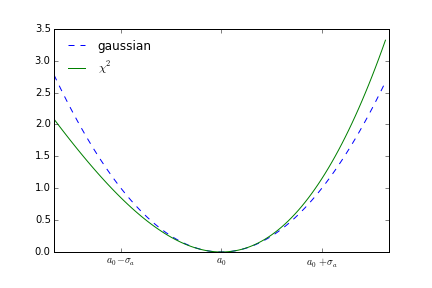
\includegraphics[width=0.75\textwidth]{figs/chisq.png}}
\end{center}
\caption{\label{fig:chisq} Approximation of $\chi^2$ near minimum.}
%x = np.arange(0,10,0.1)
%y = (x - 5)**2/3**2
%z = y + 0.05*(x - 5)**3/3**2 
%plt.plot(x,y,"--",label="gaussian")
%plt.plot(x,z,"-",label="$\chi^2$")
%plt.legend(loc=2,frameon=False)
%plt.xticks([2,5,8],["$a_0 - \sigma_a$", "$a_0$", "$a_0 + \sigma_a$"])
%plt.savefig("chisq.png")
\end{figure}

{\bf Exercise} Show that at the minimum, varying a parameter by it's uncertainty changes the $\chi^2$ by 1.

\subsection{Numerical Least Squares Fitting}

The $\chi^2$ formalism lends itself easily to numerical solutions, since the problem amounts to the optimization problem of finding the minimum of a function.  A popular approach is the gradient descent approach.  The minimum is approached in steps, with the gradient calculated at each step, and used to point the direction of the next step.  The size of the step can be chosen so that the gradient is approximately constant during the step, such as by estimating the second derivative.  Once at the minimum, the uncertainties can be estimated from the second derivative according to Equation~\ref{eqn:chisqunc}.

The major limitation of the steepest descent approach is that it will generally find only the nearest {\em local} minimum.  There is no guarantee that the global minimum has been reached.  This limitation is generally avoided by making an initial guess which is known to be near the actual minimum.  Also, the results of fits should always be evaluated to make certain they are sensible... local minimums that are not the absolute minimum almost always look ridiculous when plotted against the data!

A complete example implementing a straight line fit in scientific python is included below.  Note a few snippets in particular:
\begin{verbatim}
def func(x, a, b):
    return a*x + b
popt, pcov = curve_fit(func, x, y, sigma=yunc, p0=[1,1],absolute_sigma=True)
\end{verbatim}
The fit function is the user defined function "func", which in this case, takes two parameters ($a$ and $b$).  The call to curve\_fit is where the actual fit is performed.  Notice that the uncertainties are provided explicitly, the initial guesses are provided, and the uncertainties are specified as absolute.

The default behavior of curve\_fit is rather unscientific and intended for the general public.  It simply assumes all uncertainties are equal (if sigma is unspecified) and scales the uncertainties by an amount that gives a reasonable $\chi^2$ at the minimum.  This is seldom what a physicists wants.

You obtain the fitted parameters and their uncertainties from the return values of the functions:
\begin{verbatim}
# report the fitted values:
print "fitted values:  ", popt

# report the uncertainties, determined from the diagonals of the covariance matrix:
perr = np.sqrt(np.diag(pcov))
print "statistical uncertainties:  ", perr
\end{verbatim}
The non-diagonal elements are beyond the scope of this course, but generally provide information about how the fit parameters are correlated.  Generally speaking, highly correlated parameters should be avoided by choosing a more appropriate parameterization.

The full example is here:

\begin{verbatim}
#
# fiteg.py
#
# An example program for fitting a straight line to data with uncertainties:
# 

import matplotlib.pyplot as plt
import numpy as np
from scipy.optimize import curve_fit

# generate simulated data y = a*x + b according to:
a = 3;
b = 5;
x = np.arange(0,10)
y = a*x + b
yunc = 0.5 + y*0.03
# smear data by the uncertainties yunc
y = y + np.random.normal(scale=yunc)

# plot the simulated data with uncertainties:
fig, ax = plt.subplots(1,1)
ax.set_xlabel('x')
ax.set_ylabel('y')
ax.errorbar(x,y,yunc,fmt="ko")

# fit the data to the straight line implemented in "func":
# note we provide explicitly:
# - the uncertanities on y (sigma = yunc)
# - the starting guess for our parameters (p0=[1,1])
# - we specify the sigmas are absolute, not just relative, when determining statistical 
#   uncertainties (absolute_sigma=True)  A good test is to set this False and make 
#   certain it doesn't dramatically change your results, which would be evidence that 
#   either your uncertainties are inaccurate or the model is poor.

def func(x, a, b):
    return a*x + b
popt, pcov = curve_fit(func, x, y, sigma=yunc, p0=[1,1],absolute_sigma=True)

# report the fitted values:
print "fitted values:  ", popt

# report the uncertainties, determined from the diagonals of the covariance matrix:
perr = np.sqrt(np.diag(pcov))
print "statistical uncertainties:  ", perr
\end{verbatim}

\section{Appendix:  The Central Limit Theorem}

First we'll need to define the characteristic functions of a probability distribution function (PDF), which is simply the expectation value of the complex exponential:
\begin{equation*}   
\phi(t) \equiv \braket{\exp(itx)}  
\end{equation*}  
this is, equivalently, just the Fourier Transform of the PDF:
\begin{equation*}
\braket{\exp(itx)} = \int_{-\infty}^{+\infty} dx \; p(x) \exp(itx)
\end{equation*}
The characteristic function of a Gaussian PDF with $\sigma=1$ and mean value $\mu=0$ is then:
\begin{eqnarray*}
\phi(t) &=& \braket{\exp(itx)}\\
&=& \int_{-\infty}^{+\infty} dx \; \frac{1}{\sqrt{2\pi}} \exp\left(-\frac{x^2}{2}\right)\exp(itx)\\
&=& \int_{-\infty}^{+\infty} dx \; \frac{1}{\sqrt{2\pi}} \exp\left(-\frac{x^2-i2tx}{2}\right)
\end{eqnarray*}
And now completing the square by noting:
\begin{eqnarray*}
(x-it)^2 &=& x^2 - i2tx + (it)^2 
\end{eqnarray*}
so that the characteristic function is:
\begin{eqnarray*}
\phi(t) &=& \int_{-\infty}^{+\infty} dx \; \frac{1}{\sqrt{2\pi}} \exp\left(-\frac{(x-it)^2+(it)^2}{2}\right)\\
&=& \exp\left(\frac{1}{2}t^2\right)\int_{-\infty}^{+\infty} dx \; \frac{1}{\sqrt{2\pi}} \exp\left(-\frac{(x-it)^2}{2}\right)
\end{eqnarray*}   
where the integral is now simply the integral of a Gaussian distribution (albeit one with a complex mean value) which integrates to simply 1.  And so the characteristic function of the Gaussian distribution is:
\begin{equation}
\phi(t) = \exp\left(\frac{1}{2}t^2\right) \label{eqn:cfn}
\end{equation}
 The proof of the Central Limit Theorem amounts to showing that the characteristic function of a sum of random variables, from any PDF, with finite variance converges to the characteristic function for the Gaussian distribution.  Due to Levy's Continuity Theorem, the proof of which we'll leave to the mathematicians, this means that the PDF for the sum of random variables converges to the Gaussian distribution.

We can assume, without losing generality, that we have $n$ independent random variables $x_i$ identically distributed with mean $\mu=0$ and $\sigma=1$.  We consider the random variable $z$ which is the sum of these random variables:
\begin{displaymath}
z = \frac{1}{\sqrt{n}}\sum x_i 
\end{displaymath}
The expectation value for a function of $z$ is therefore an integral over all of the $x_i$ variables each weighted by the PDF:
\begin{equation}
\braket{f(z)}_z = \int \; \left( \prod_i dx_i \; p(x_i) \right) \; f\left( \frac{1}{\sqrt{n}}\sum x_i \right) 
\end{equation} 
 The characteristic function of the random variable $z$ is therefore:
\begin{eqnarray*}
\phi(t) &=& \braket{\exp(itz)}_z \\
           &=& \int \left( \prod_i dx_i \; p(x_i) \right)  \exp\left( \frac{it}{\sqrt{n}}\sum_i x_i \right) \\
           &=& \int \left( \prod_i dx_i \; p(x_i) \right)  \left( \prod_i \exp\left(\frac{itx_i}{\sqrt{n}}\right) \right)\\           
           &=& \prod_i \int dx_i \; p(x_i) \exp\left(\frac{itx_i}{\sqrt{n}}\right) \\                      
           &=& \prod_i \braket{\exp\left(\frac{itx_i}{\sqrt{n}}\right)} \\
           &=& \left[\braket{\exp\left(\frac{itx}{\sqrt{n}}\right)}\right]^n
\end{eqnarray*}
where in the last step we have used the fact that the $x_i$ are identical independent random variables.  Now expanding the exponential as a Taylor series:
\begin{eqnarray*}
\phi(t) &=& \left[\braket{1 + \frac{it}{\sqrt{n}}x+\frac{(it)^2}{2n}x^2+\ldots}\right]^n\\
&=& \left[1 + \frac{it}{\sqrt{n}}\braket{x}+\frac{(it)^2}{2n}\braket{x^2}\right]^n \\
&=& \left[1 -\frac{t^2}{2n}\right]^n
\end{eqnarray*}
 Now in the limit $n \to \infty$ this becomes:
\begin{eqnarray*}
\phi(t) &=& \lim_{n \to \infty} \left[1 -\frac{t^2}{2n}\right]^n \\
          &=& \exp\left( \frac{1}{2}t^2\right)
\end{eqnarray*}
which is the characteristic function from the Gaussian distribution.


\end{document}




